\section{Background} \label{background}

\subsection{Haskell \& Functional Programming}
Functional programming differs from imperative programming in many ways. The building blocks of functional languages are their namesake, functions, and in their basis, the lambda calculus, there are no values except functions. Functional languages extend the lambda calculus with types, functions names, and more, but at their core can be represented by plain untyped lambda functions.
\subsubsection{Lazy Evaluation}
Many common languages are ``strict'', using call-by-value evaluation strategy. When a value is parsed into a function, it is first evaluated, regardless of it is actually used or not. This comes with the benefits of reduced complexity, and more intuitive control flow.
\begin{figure}[b]
    \centering
\begin{lstlisting}[language=Python]
x = [print("First"), print("Second")]
\end{lstlisting}
    \caption{A strict language would print 'First' and 'Second'\, whereas a lazy language would not.}
    \label{fig:print}
\end{figure}
On the other hand, Haskell is a ``lazy'' language, using call-by-need evaluation strategy, only evaluating expressions when necessary. Computation is stored within ``thunks'', which know how to compute their value, but are only evaluated when their value is needed. This freedom allows computation, that could otherwise never terminate, to be ignored or only partially computed, such as in Figure \ref{fig:strict-lazy}.
In some cases, this can improve performance and memory usage, especially in the cases of non-terminating thunks or infinite lists, in practice this can vary, as there is a not insignificant overhead to store closures and computations \cite{Jones_1992, Efficient_Lazy}.
However this complicates side effects such as IO. In code such as Figure \ref{fig:print} it's possible for neither, only one, or both print statements to execute depending on the rest of the code and what elements are evaluated. If the values are required, and evaluated, they will print. Otherwise, they will remain as unevaluated thunks.
\begin{figure}[t]
    \centering
\begin{lstlisting}[language=Python]
def foo(a):
    return 1
x = foo(loopforever())
\end{lstlisting}
    \caption{A strict language would hang, whereas a lazy language would return a thunk that can evaluate to the value 1.}
    \label{fig:strict-lazy}
\end{figure}

Call-by-need evaluation strategy differs slightly from call-by-name evaluation strategy, as each argument is memoized to reduce duplicate computation and side effects. It combines the benefits of call-by-value evaluation, the removal of duplicate code execution, and call-by-name evaluation, the removal of unnecessary code execution. Call-by-need evaluation also fixes cases where side effects are duplicated, such as in Figure \ref{fig:side-effects}
\begin{figure}[t]
    \centering
    \begin{lstlisting}[language=Python]
def foo(x):
    return x * x
foo(input())\end{lstlisting}
    \caption{A call-by-name language would require two user inputs, whereas a call-by-need language would require one user input, and use it twice.}
    \label{fig:side-effects}
\end{figure}

\subsubsection{Type Classes \& Monadic IO}
Haskell does not allow for function overloading, where a function can have different type signatures, and different uses depending on the arguments passed in, such as in Figures \ref{fig:overloading} and \ref{fig:overloading-2}. To conform with the strict type system, the type of the overloaded method is defined within the type class, and instances must adhere to it to compile.

\begin{figure}
    \centering
    \begin{lstlisting}[language=Java]
static int foo(int x, int y) {
    return 2 * x + y;
}
static float foo(float x, float y) {
    return x + 2 * y;
}\end{lstlisting}
    \caption{An int passed into ``foo'' will have different behaviour to a float.}
    \label{fig:overloading}
\end{figure}

\begin{figure}
    \centering
    \begin{lstlisting}[language=Haskell]
class Fooable a where
    foo :: a -> a -> a
instance Fooable Integer where
    foo x y = 2 * x + y
instance Fooable Float where
    foo x y = x + 2 * y
\end{lstlisting}
    \caption{Figure \ref{fig:overloading} rewritten using Haskell's type class system.}
    \label{fig:overloading-2}
\end{figure}

Haskell handles IO by using a variety of concepts from category theory, functors and monads. By restricting IO, and it's side effects, to within a particular data type that implements these classes. This doesn't solve the problem of indeterminate ordering, but does force the programmer to consider IO whenever handling it.
\begin{lstlisting}[language=Haskell,caption={The Functor and Monad typeclass.\protect\footnotemark.}]
class Functor f where
    fmap :: (a -> b) -> f a -> f b
class Monad m where
    (>>=) :: m a -> (a -> m b) -> m b
    (>>) :: m a -> m b -> m b
    return :: a -> m a
    fail :: String -> m a
\end{lstlisting}
\footnotetext[1]{GHC's dialect has the Monad class depend on Applicative, which depends on Functor. This differs from the Haskell 2010 Language Report which this project is based off.}
``fmap'' allows functions that were originally not designed for wrapped types, to work as intended, and the ``$>>$='' and ``$>>$'' function allows for cleanly passing wrapped types around and handling error values.
By using these operators side effects that affect the system the program runs on, including potential errors, are contained and handled appropriately. A variety of other functions exist with the standard library to help use these classes easily.

These classes are also used elsewhere, especially for simple error handling. For example, in Listing \ref{safeHead}, if the first call to "head" returns Nothing, it is propagated onwards. Only if both the calls to "head" return values does it return a tuple of the values.
\begin{lstlisting}[language=Haskell, caption=Safely fetch the first two elements of a list., label=safeHead]
head :: [a] -> Maybe a
head [] = Nothing
head (x:_) = return x

dualHead xs =
    head xs >>=
    \x -> head (tail xs) >>=
    \y -> return (x,y)
\end{lstlisting}
Numerous other built-in functions use the Maybe and Either types for malformed arguments, such as for safe division, which then must be handled by the caller through pattern matching or the class methods. This allows many errors, such as division by zero which would throw an error in most other languages, to be handled safely before the program ever runs. The programmer is unable to simply overlook the error and cause a program crash during runtime.

\subsection{Visualisation}
\label{visualisationsection}
Various visualisers exist online for visualising algorithms, data structures, as well as general programming languages. Countless YouTube videos exist breaking down algorithms and data structures step by step to explain how they work, and sites like \cite{algo-vis} have a wide array of algorithms and data structures that can be viewed.

More focused, visualisers can also show general programming languages. Especially for imperative languages, the current memory can be tracked \cite{cscircles-vis}, showing what values exist in memory, and what variables represent what values. This is especially common in debuggers, such as the one's built into modern web browsers to aid with JavaScript development, such as the one shown in Figure \ref{fig:chrome}. These types of visualisers can greatly aid in development, as the exact line of code where the problem occurs can be quickly detected.
\begin{figure}[t]
    \centering
    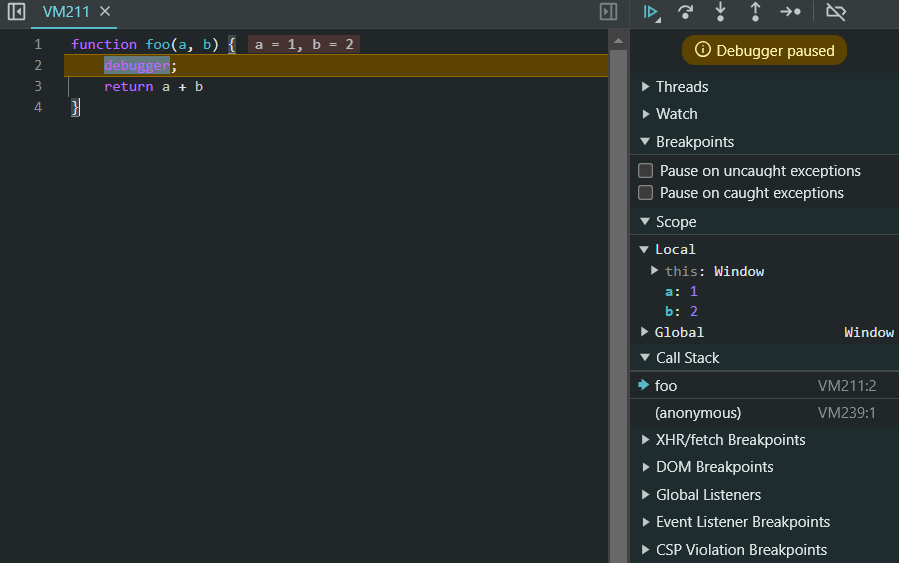
\includegraphics[width=1\linewidth]{chapters/2-background/figures/debugger.png}
    \caption{Google Chrome's debugger, showing the current state in code, including bound variables, including implicit variables, such as ``this''.}
    \label{fig:chrome}
\end{figure}

Visualisers come in many different styles, some such as Google Chrome's debugger are largely plain and text-based, aiming to be user friendly without knowledge of how the language works behind the scenes. The extreme end of this are visualisers like \cite{visualize-cbn}, which, at every step of evaluation, shows a valid Haskell expression. This visualiser is especially adept at visualising lazy evaluation, as each step transforms into a new valid with only the relevant changes, allowing the user to see which thunk has been evaluated.

Other visualisers opt for a graph based approach, such as the \cite{SPARTAN} visualiser by Waugh Ambridge. These types of visualisers are often much lower level, in this case showing individual applications, bindings, as well as showing when and which thunks are being evaluated. These types of visualisers require more in depth knowledge of the basis of functional programming, lambda calculus, as they remove most of the abstraction and simplicity gained from the programming language syntax.

\subsection{User Study}
\subsubsection{Motivation}
To gauge how useful such a visualiser would be, an online survey was designed to work out how effective the current methods of teaching functional programming had been. Singer and Archibald \cite{singer2018functional} had shown that there were significant challenges to learning functional programming, with frequent errors preventing code execution. The survey would help validate the need for more tools and visualisers within functional programming. It would also be useful to know which methods were commonly used to help debug programs, and to analyse them to work out how they help, and how they could be improved.

The survey was aimed towards students either currently in their 2$^{nd}$ year (when the Functional Programming module is taught at the University of Birmingham), and those in later years who had already taken the module. 14 students responded, 3 in their 2$^{nd}$ year and 11 in later years.

\subsubsection{Results}
Not all the questions in Appendix \ref{survey} were required, but enough responses were recorded to show the need of a tool to help learn and debug Haskell. All the answers are also recorded in Appendix \ref{survey}.
\\\\\textbf{Which tools/visualisers have you used for testing and debugging Haskell?}\\
If users were already familiar with an existing suite of tools to help learn Haskell, the usefulness of a new one would be greatly diminished. 
Of the responses, 10 participants said they hadn't used any tools for helping with Haskell. 3 participants used GHCi, an interactive shell built by the GHC contributors. It is capable of showing the principle type of expressions, and is the easiest way to run functions as scripts. 1 participant reported using the Haskell extension available within the VSCode marketplace. This extension is widely used, with over half a million downloads, and comes with a large number of functions including type checking expressions as the user implements them, allowing errors to be detected without having to attempt compilation.
\\\\\textbf{Which tools/visualisers have you used for testing and debugging other languages?}\\
In contrary to Haskell, tools among other languages are much more common. 5 participants reported using a variety of VSCode extensions for languages, which includes linters, debuggers, and type checkers. A number of other debuggers, GDB for C, PyCharm, mypy, ruff, and more for Python, and a variety of Java tools were mentioned by them and other respondents.
Only 3 participants didn't report using any tools to test and debug, a sharp drop from Haskell.
It's clear that Haskell has a much smaller array of tools available when compared to other languages, and those that do exist are used much less frequently and are often less comprehensive than other tools.
\\\\\textbf{How did you find the transition from object-oriented imperative languages to a functional language? (1-5, hard-easy)}\\
The average response to this question was 3.4 out of 5, indicating that the transition wasn't really easy, but also wasn't really hard. As shown below, I think this is because some concepts, such as higher order and anonymous functions, are already present in a number of popular languages, and are fairly well understood, whereas the more complicated concepts can typically be ignored until the user needs to implement a function using them.
\\\\\textbf{How well would you say you understood the following concepts? (1-5, not well-very well) (Additional comments in Table \ref{tab:comments})}\\
Participants were asked about higher order functions, anonymous functions, monads, lazy evaluation, partial application, and pure functions. As expected, the concepts common to other languages, higher order and anonymous functions, on average scored higher, 4.2 and 4.3 out of 5 respectively.
When leaving out participants who responded that they did not know what the concept was, the remaining concepts, in order from most to least well understood, were lazy evaluation (4.0/5), partial application (3.6/5), pure functions (3.5/5), and monads (2.8/5).
When asked to elaborate on difficulties, several respondents reported they only felt like that had a surface level understanding of concepts. "\textit{I...never fully understand WHY they worked or were a certain way.}", "\textit{I still didn’t find them [monads] intuitive.}". This could be due to users being unable to see how these concepts actually evaluate, which could be rectified with a step by step visualiser, such as what this project aimed to achieve.
\\\\\textbf{How likely are you to use a functional language in the future?} (Answers in Table \ref{tab:future})\\
6 respondents said they were likely, 4 said they were unlikely to use functional programming in the future, and 2 said they would use some concepts in their imperative programming.
The elegance and correctness of functional programs was noted as a positive, as well as being able to emulate the notation of mathematics within programs. The lack of tooling, and familiarly with imperative object-oriented programming was noted as reasons to not continue with functional programming.

\subsubsection{Analysis}
Despite the small number of participants, it's clear that Haskell lacks the extensive tooling that is present in many other popular languages. Many of the responses reflect my own feelings regarding functional programming. This validates the aim of this project, and its success will be partially dependant on how users are able to use the visualiser to improve their understanding of Haskell.